\begin{figure}
    \centering
    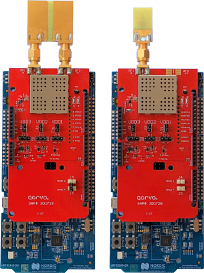
\includegraphics[width=0.2\textwidth]{images/QM33120WDK1_PDP_v2.png}
    \caption{QM33120WDK1 Ultra-Wideband (UWB) Transceiver Development Kit. The Nordic nRF52840DKs (the blue boards behind), are the actual companion boards on which the firmware runs.}
    \label{SEN:fig:eval_kit}
\end{figure}

As already underlined, for the target position estimate, we have used the Ultra-Wideband (UWB) Transceiver Development Kit produced by Qorvo \autoref{SEN:fig:eval_kit}, for which we refer to the official website page\cite{UWBQorvo} for details and datasheet\cite{UWBDatasheet}. For this kit, is also available a firmware that can be requested from Qorvo. Reading the code, we have deduced the following main information:
\begin{itemize}
    \item AoA and distance, are fed directly to the serial port in an encoded string with other quantity like PDoA, status and block number;
    \item The firmware can run in different configurations, depending on the antenna type and the selected communication channel\footnote{The channel type, allows to change between the two supported IEEE standards: IEEE Std. 802.15.4™‐2020\cite{IEEEstd_4} and IEEE Std. 802.15.4z™‐2020\cite{IEEEstd_4z}}: \textit{Jolie} and \textit{Monalisa} are the two antenna types. The possible channels are instead $9$ and $5$. It follows that the antenna can be configured in $4$ different ways, using the parameter \texttt{ANTENNA}: \texttt{JOLIE9}, \texttt{JOLIE5}, \texttt{MONALISA9}, \texttt{MONALISA5}. Our antenna is a \textit{Jolie} and the default channel is $9$, meaning that the \texttt{ANTENNA} parameter is equal to \texttt{JOLIE9} by default. 
    \item PDoA raw measures, are adjusted by means of a stepped linear regression. The steps of this linear regression are defined by a pair of look up table (different for each channel and antenna type): one for the PDoA intervals, and one for the slopes that the liner regression model has to have inside these intervals. All the values were clearly calculated after laboratory test, aiming to reduce the non linear effects present in the raw PDoA measure; 
    \item The PDoA value truly used to calculate AoA by means of the relation \eqref{PRFOR:eq:aoa-pdod}, is the average of the last \texttt{PAVRG} values, corrected with \texttt{PDOAOFF}. \texttt{PAVRG} and \texttt{PDOAOFF} are user definable constant by default equal to $10$ and $0$ respectively. The first defines the values over which perform the moving average: an high value can mitigate the high frequency error, but can worst the sensor performance in detecting PDoA change; on the other side a lower value can detect even rapid changes in the actual PDoA, but the high frequency error contribution is not lowered. \texttt{PDOAOFF} defines instead the offset to apply at the average result as a user calibration.
\end{itemize}

\begin{figure}
    \centering
    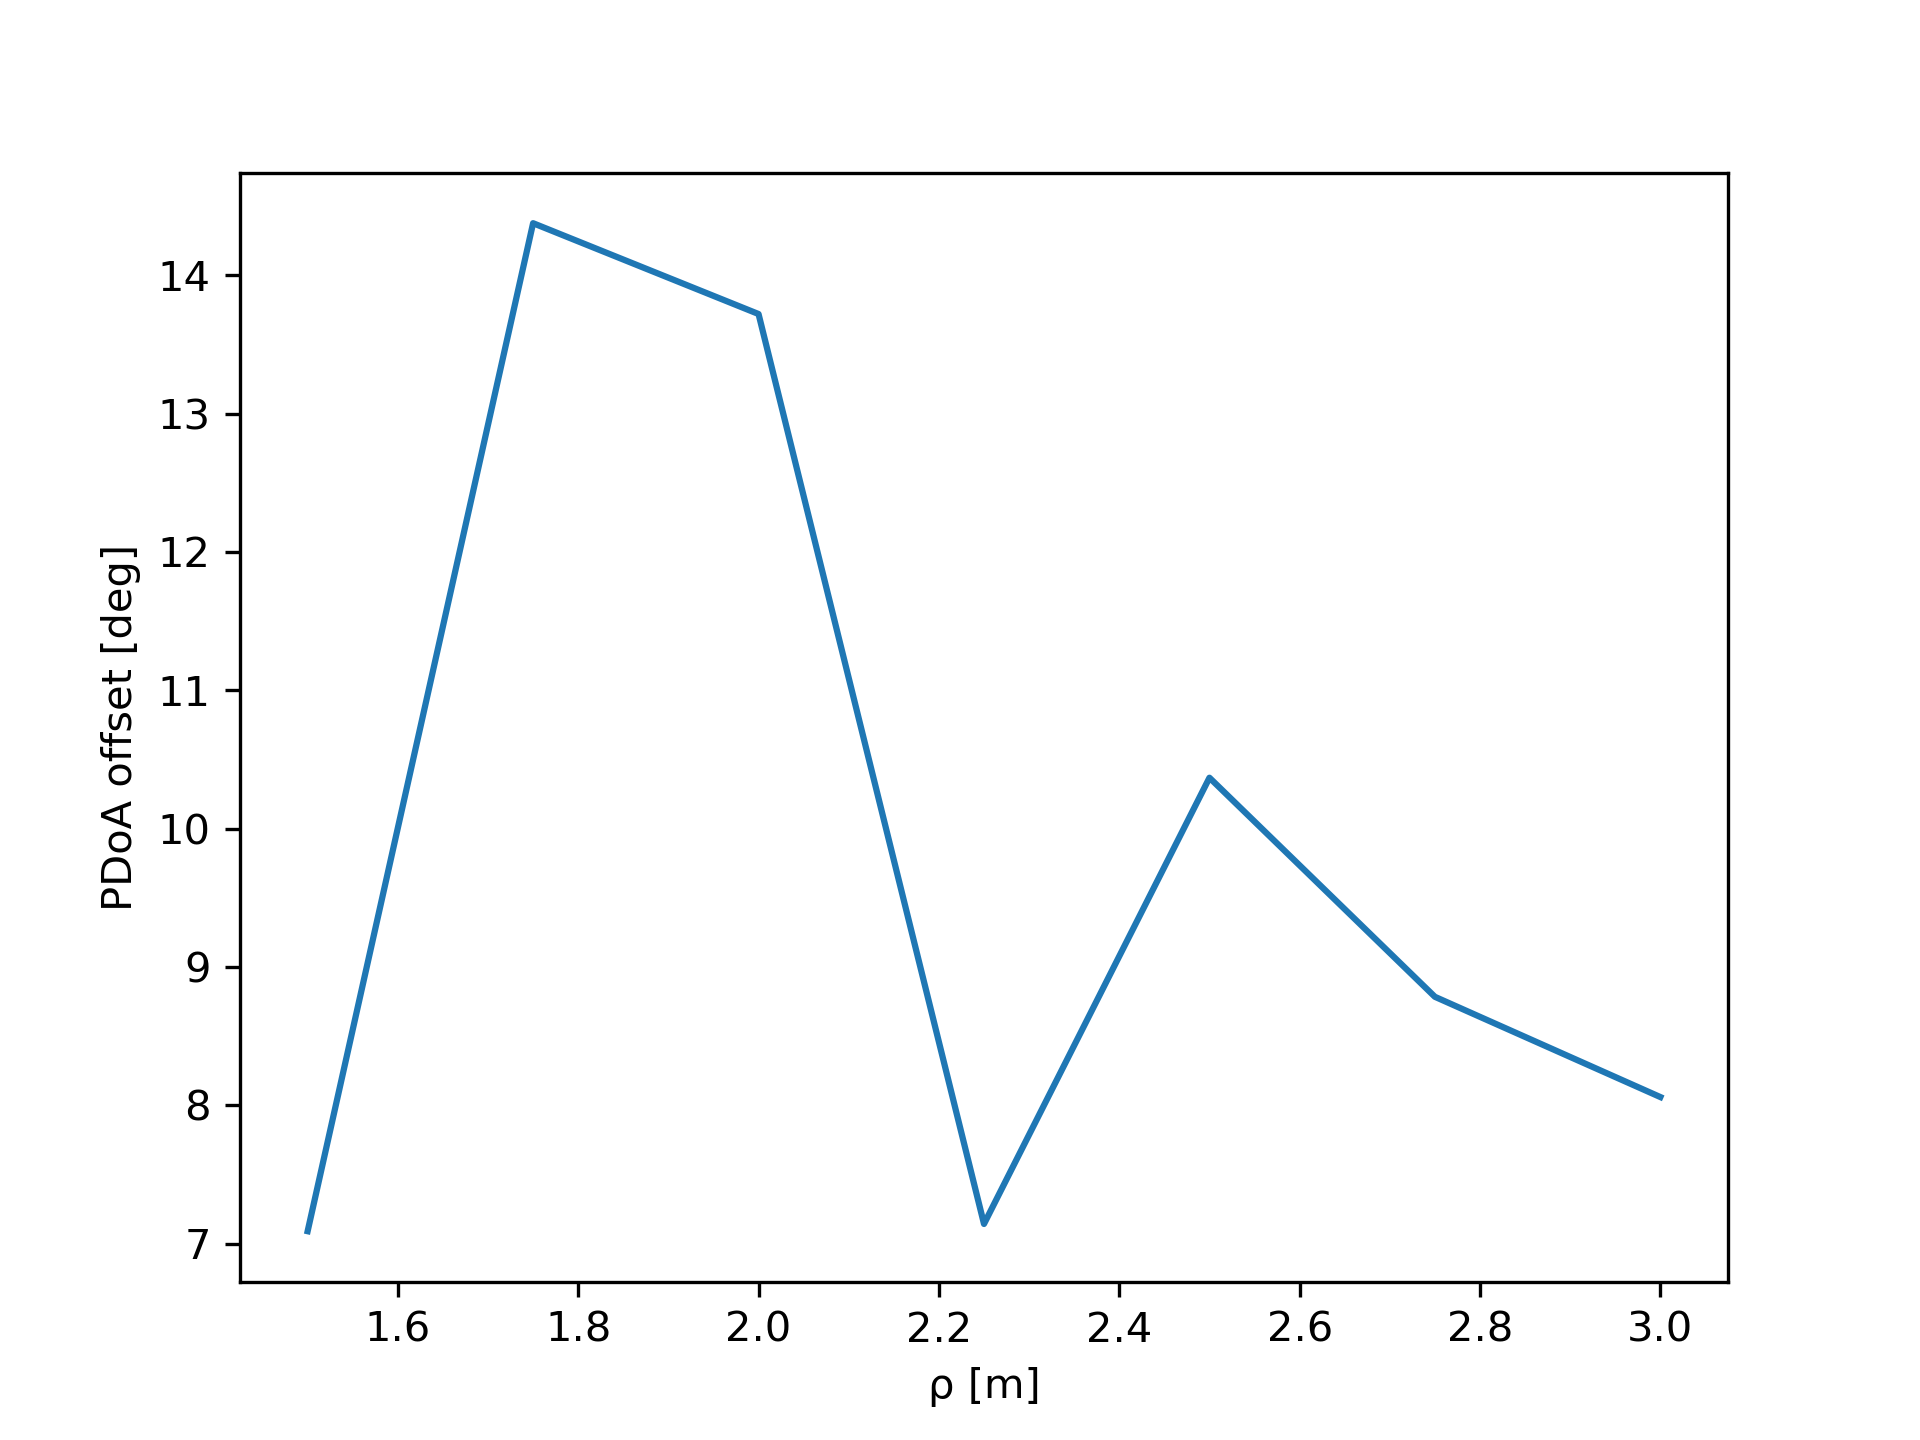
\includegraphics[width=0.45\textwidth]{images/PDOAOFF_trend.png}
    \caption{\texttt{PDOAOFF} at various distances.}
    \label{UWB:fig:PDOAFF}
\end{figure}

\subsection{Characterization}
In order to understand the behavior of the above kit, we have performed a sensor characterization to asses what follows:
\begin{itemize}
    \item Performance difference using the two supported IEEE standards (i.e. channel $9$ or $5$), comparing the results at different angles and distances;
    \item Performance at different tag heights and angles;
    \item Result obtained, by putting the tag behind the double-UWB anchor;
\end{itemize}
Since the first tested channel configuration was the default one (i.e. $9$), the last two results were extracted only for this configuration. By the way, channel type should not change noticeably the validity of the extracted information (e.g. if the kit performance are worsen by a tag height change, the channel should not be a discriminant).\\
All the listed assessment, where performed using MoCap as ground truth and even for precise positioning (i.e. to place the tag at precise distances, angles and eventually heights w.r.t the double UWB).\\

\begin{figure*}
    \centering
    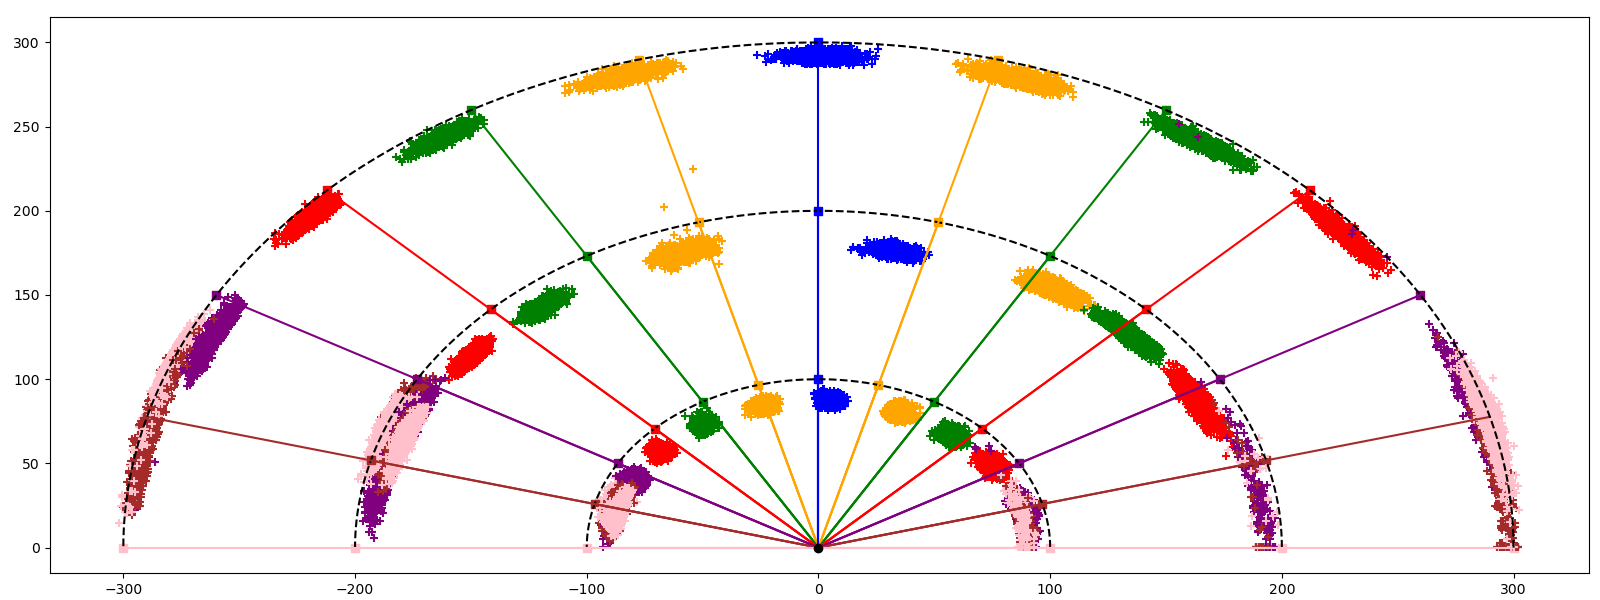
\includegraphics[width=1.0\textwidth]{images/ch9_characterization.png}
    \caption{Location test conducted with channel 9 standards, expressed in centimeters.}
    \label{UWB:fig:ch9test}
\end{figure*}

\begin{figure}
    \centering
    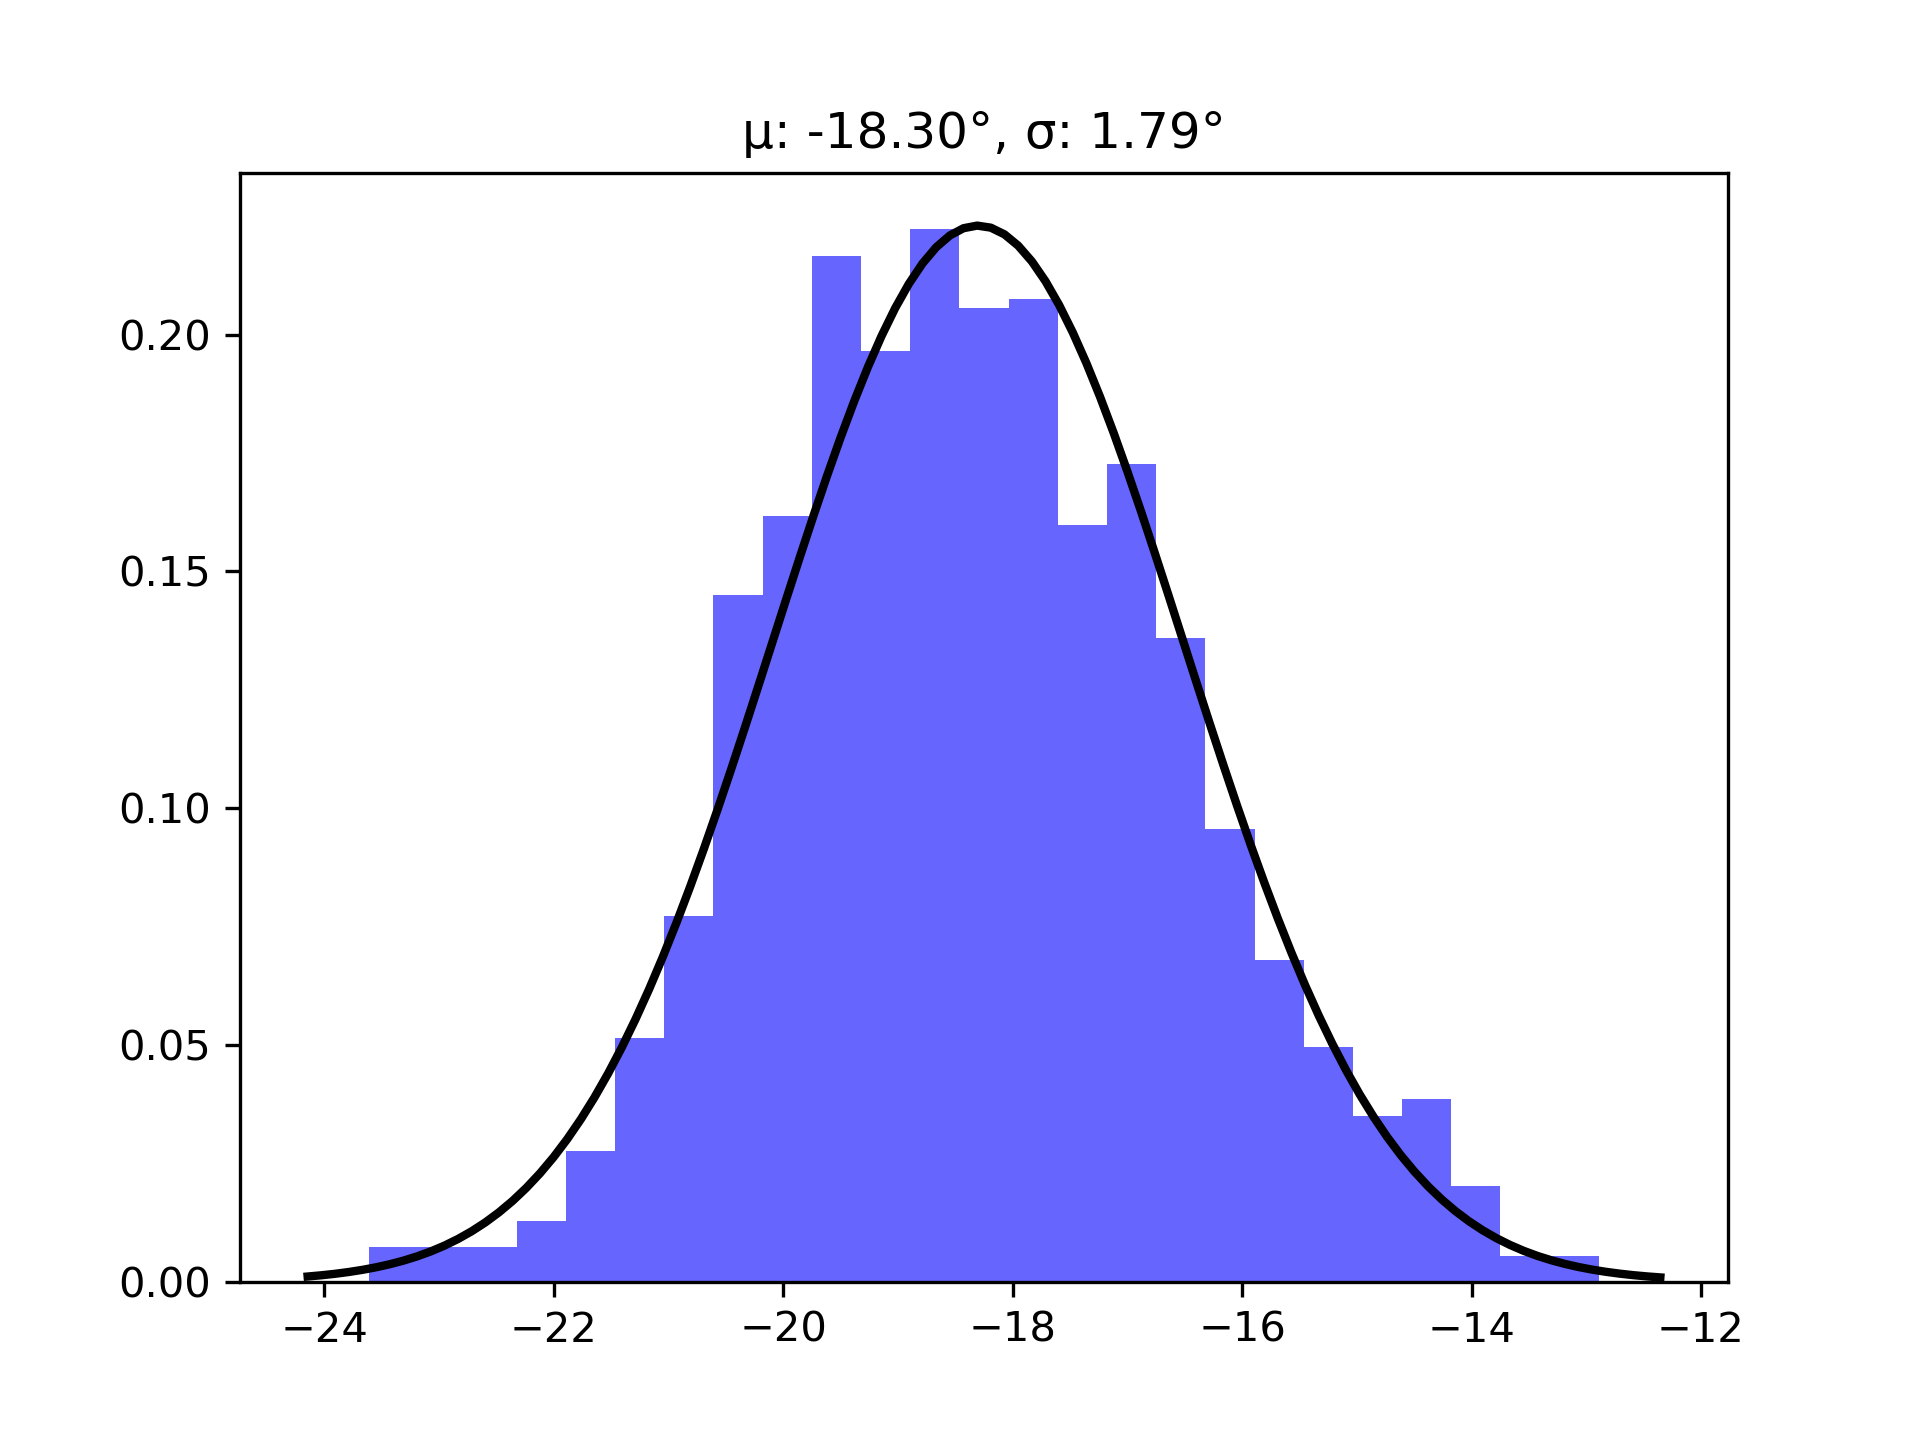
\includegraphics[width=0.45\textwidth]{images/ch9_aoa_hist.png}
    \caption{Channel 9 AoA measurements distribution at $-15$ degrees and $200$ centimeters.}
    \label{UWB:fig:AoA_ch9}
\end{figure}

Since the UWB kit declared working region is the half-plane in front of the double UWB, to compare the behaviour under the two different IEEE standards, we have perform tests in this region, at different discrete values of range and angles. Since that half-plane can be defined with a polar coordinate pair, with undefined radius and angles from $-90$ to $+90$ degree (being $0$ degree when the the tag is in front of the double), we have perform the test as follow:
\begin{itemize}
    \item For channel $9$, at three different range $\rho_9=\begin{bmatrix} 1,2,3 \end{bmatrix} [m]$, and angles from $-90$ to $+ 90$ with a step of $15 deg$;
    \item For channel $5$, at two different range $\rho_5=\begin{bmatrix} 1.5, 2.5 \end{bmatrix} [m]$ and angles from $-90$ to $+90$ for the first range and from $-60$ to $+60$ for the second, again with a step of $15 deg$
\end{itemize}

As suggested by the manufacturer, before the data collection we calibrated the PDoA offset placing the modules at a distance of at least 1.5 meters at 0 degrees, collecting 1000 measures of the PDoA, that ideally should be 0, and averaging the values to obtain the \texttt{PDOAOFF} value to set. For the channel 9 configuration, we determined it at a distance of $2.5$ meters, thinking that the range did not have much influence. However, before the channel 5 data collection, we realized that it changes with the distance, as can be seen in \autoref{UWB:fig:PDOAFF}. Hence, to setup the modules to be used at a distance congruent to the one of the following task, we identified and set the \texttt{PDOAOFF} at 1.5 meters.\\

\begin{figure}
    \centering
    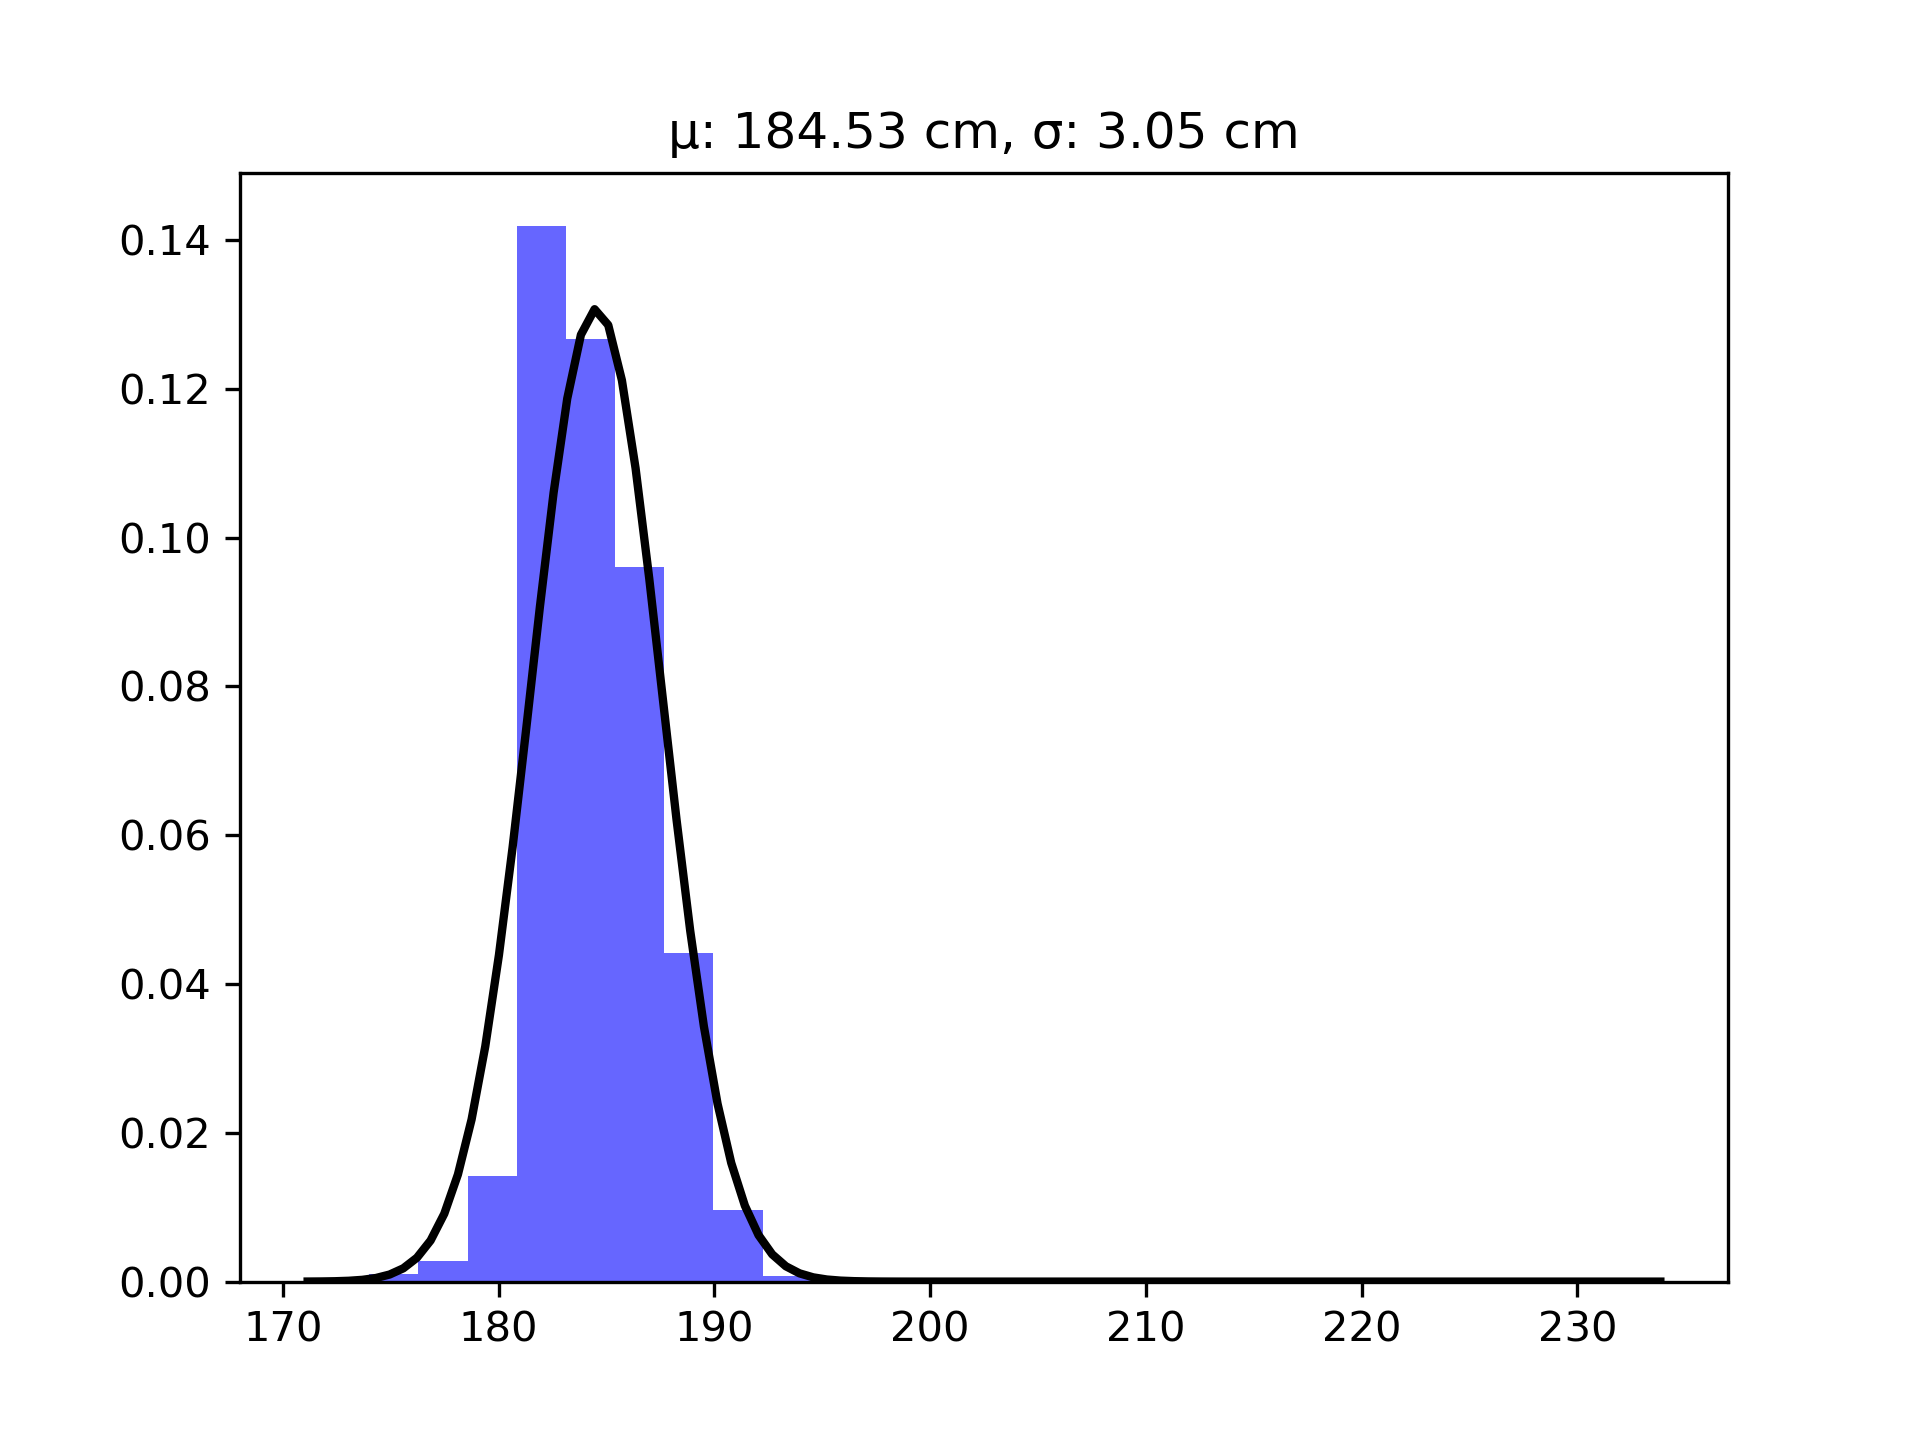
\includegraphics[width=0.45\textwidth]{images/ch9_range_hist.png}
    \caption{Channel 9 range measurements distribution at $-15$ degrees and $200$ centimeters}
    \label{UWB:fig:Range_ch9}
\end{figure}

\begin{figure*}
    \centering
    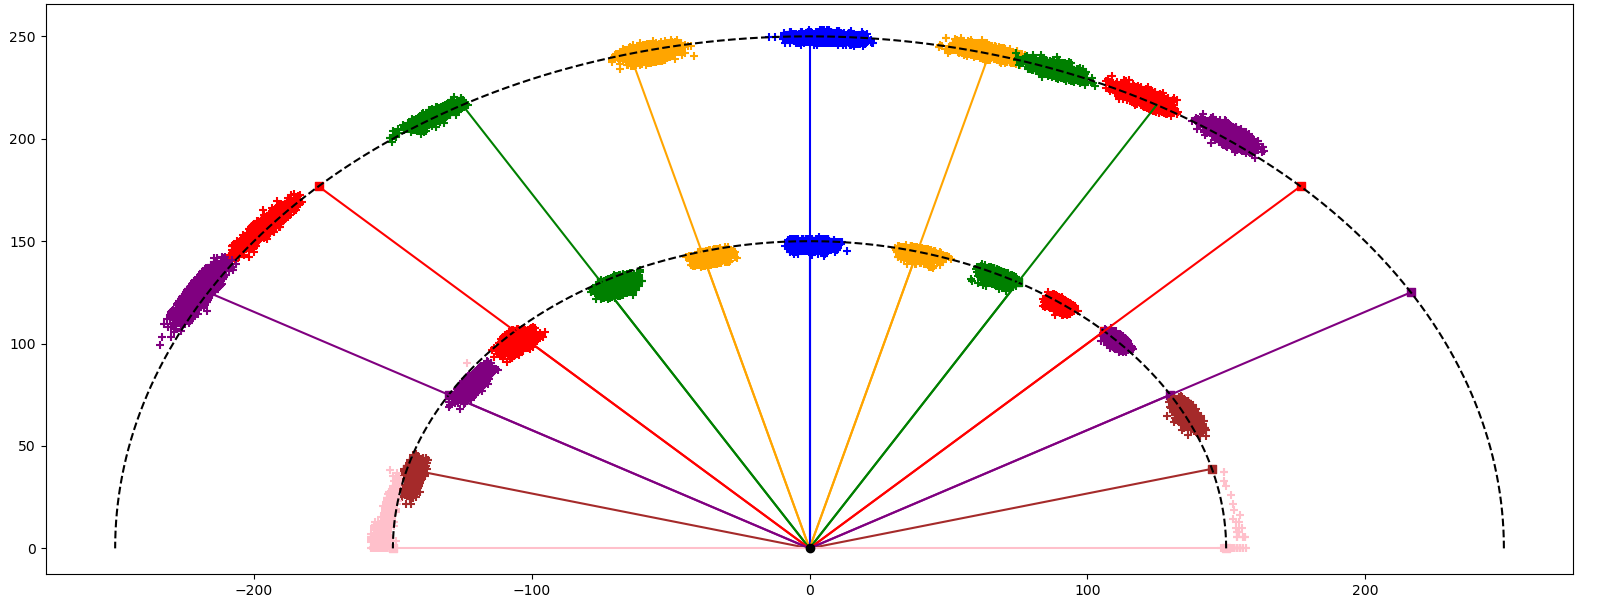
\includegraphics[width=1.0\textwidth]{images/ch5_characterization.png}
    \caption{Location test conducted with channel 5 standards, expressed in centimeters.}
    \label{UWB:fig:ch5test}
\end{figure*}

\begin{figure}
    \centering
    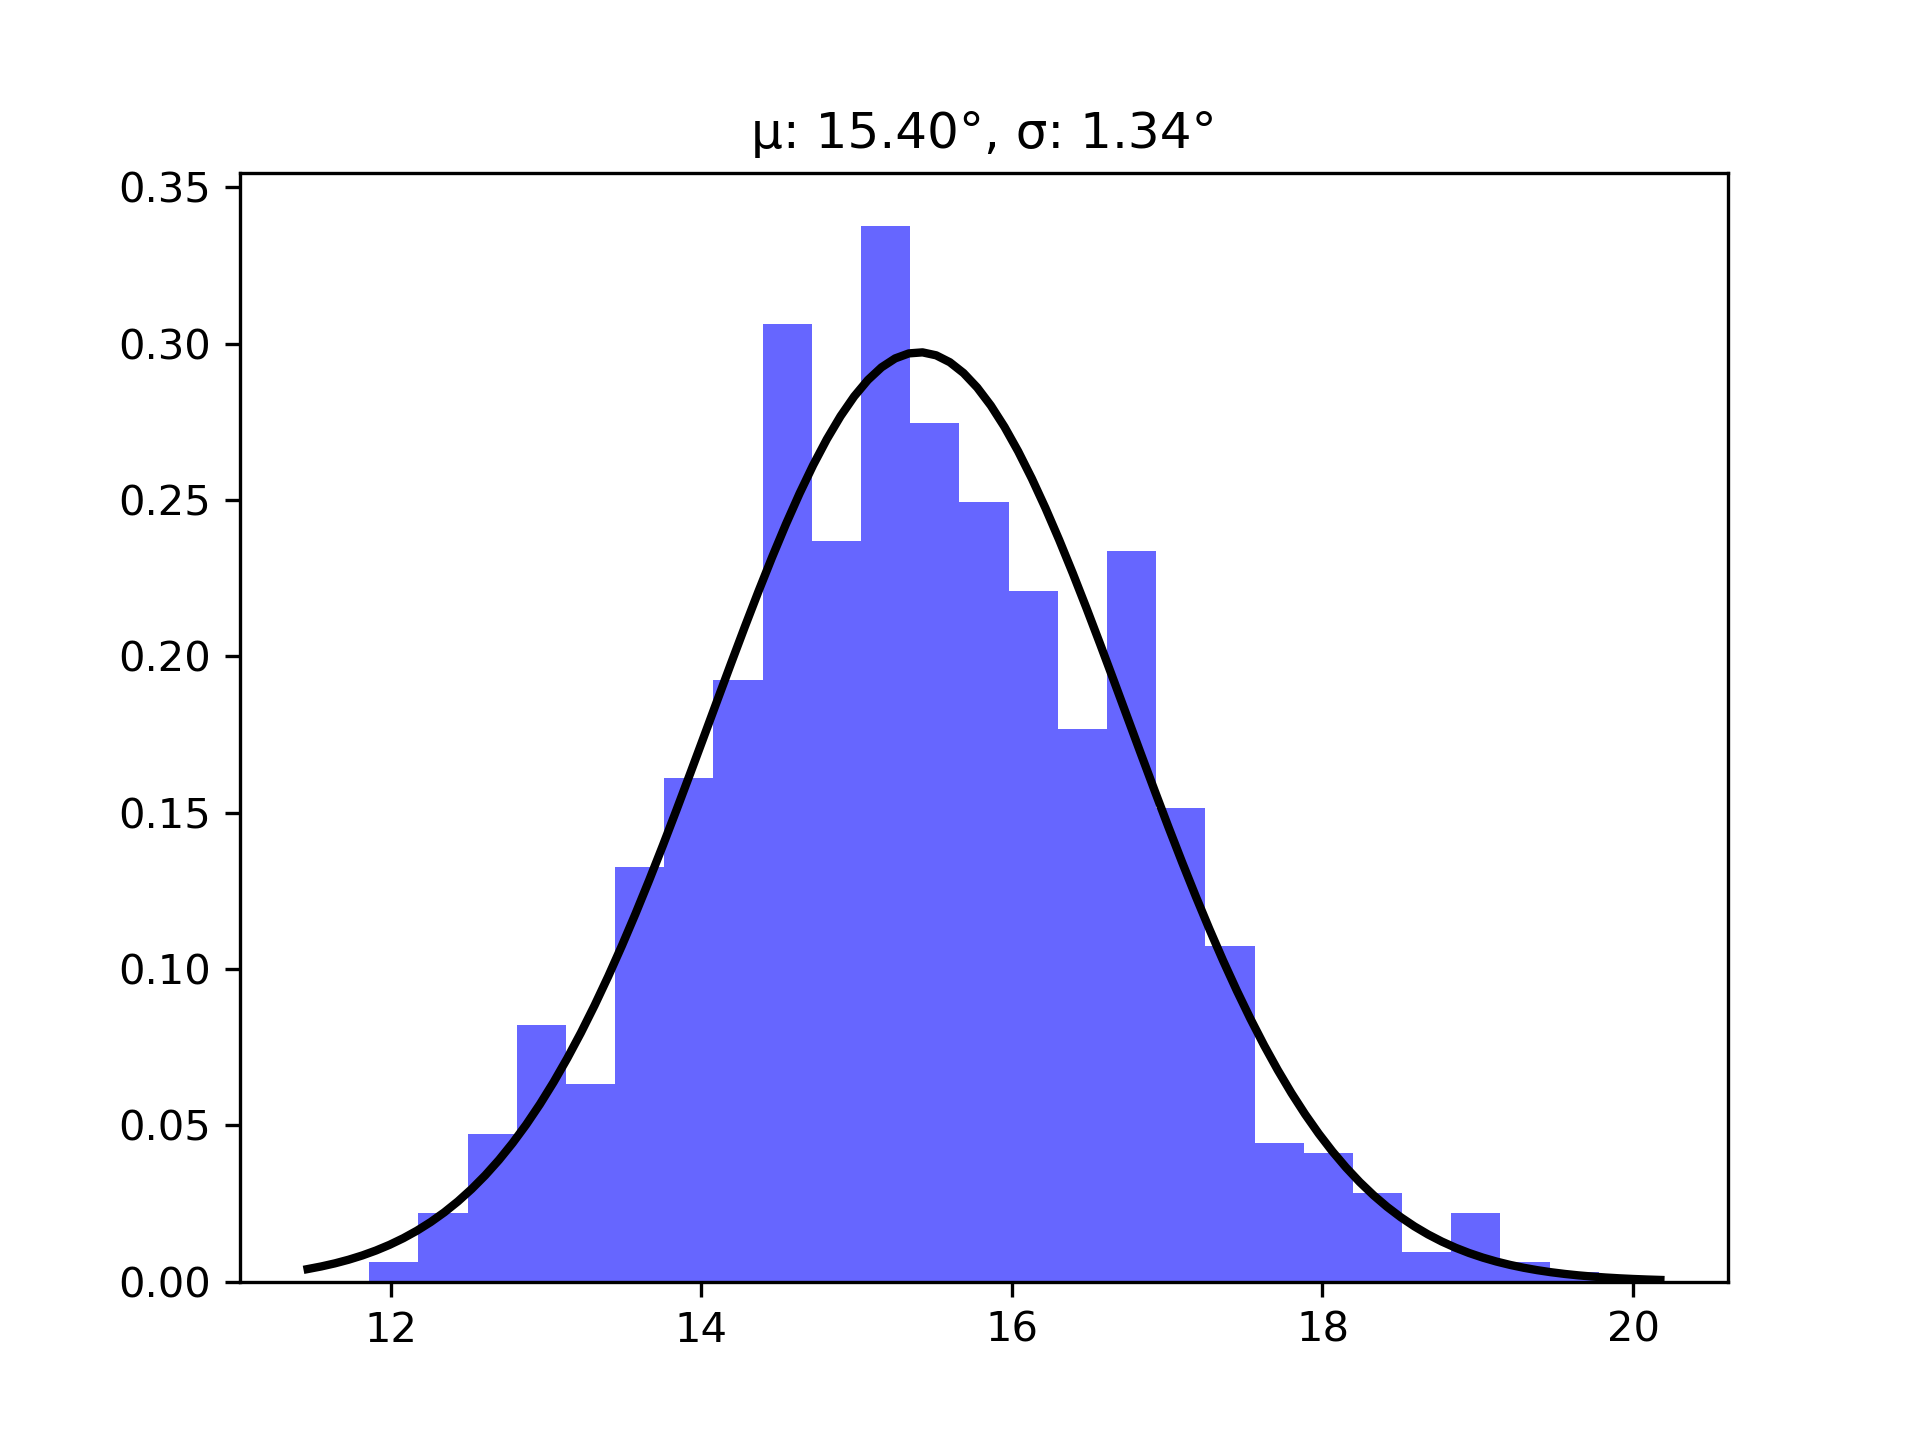
\includegraphics[width=0.45\textwidth]{images/ch5_aoa_hist.png}
    \caption{Channel 5 AoA measurements distribution at $+15$ degrees and $200$ centimeters.}
    \label{UWB:fig:AoA_ch5}
\end{figure}

\paragraph{Channel Comparison}
The tests results for channel 9, are depicted in \autoref{UWB:fig:ch9test}. The graph shows different behaviours at different distances. For example at a distance of $3$ meters the estimated angle is quite good, whereas at $2$ meters it shows different behaviours for the negative and the positive part of the half-plane. Indeed for positive angles it shows better values. Despite this, the measured angles are generally bad. This behaviour could be caused by the great variation of \texttt{PDOAFF} at $2$ meters w.r.t. $2.5$, as shown in \autoref{UWB:fig:PDOAFF}. At $1$ meter the results are slightly better, but still there is asymmetry between positive and negative part. Another characteristic  to denote, is that despite the distance, at angles greater then $75$ degree (and $-75$), the angles are not reliable and tend to be much more scattered. For what concerns the range, a not constant negative bias is always present. The data clouds, shows instead an almost constant spread, indicating that the standard deviation of both range and angles, are constants. A pair of distribution examples, are presented in \autoref{UWB:fig:AoA_ch9}, \ref{UWB:fig:Range_ch9}. Both shows a bias w.r.t. the actual angle and range, but their distributions are gaussian-like, with $\sigma_{\alpha} = 1.79$ ° and $\sigma_{\rho} = 3.05$ cm and mean error of $3.30$ ° for the angle and of $15.47$ cm for the range. Comparing these values with the specifications of the manufacturer, reported in \autoref{UWB:tab:sensorspec}, is possible to see that the standard deviation is in accordance with the declared one both for the angle and the range. For what concerns the accuracy, the angle is inside the accuracy interval declared while it is not the case for the range. However, as can be seen in \autoref{UWB:fig:ch9test}, if instead of the measurement at $2$ meters and $-15$ degrees one would consider the data at the same distance and angle mirrored, the angle would not be anymore in the accuracy interval.\\

\begin{table}
    \centering
    \begin{tabular}{ | m{1.3cm} | m{1.2cm}| m{2.1cm} | m{0.7cm} |} 
        \hline
        &  accuracy & standard deviation & Units\\ 
        \hline
        Range & $\pm $ 6 & 3 & cm\\ 
        \hline
        AoA CH9 &$\pm$ 6.25 & 2.5 & deg \\
        \hline
        AoA CH5 &$\pm$ 6.25 & 2 & deg \\
        \hline
    \end{tabular}
    \captionsetup{type=table}
    \caption{Manufacturer declared Location Accuracy Characteristics. The values are intended after calibration, measured in line of sight in a noise-free environment. See Datasheet p.17 for reference\cite{UWBDatasheet}}
    \label{UWB:tab:sensorspec}
\end{table}
The test for the channel 5, is depicted in \autoref{UWB:fig:ch5test}. As previously specified, this test was conducted by tuning the PDoA offset at a distance congruent with the one of the following task, that is $1.5$ m, in order to reduce all the error in the working region. To this end, even the tested ranges were changed to a pair $1.5$ and $2.5$ m.\\
Also for this test, the asymmetry between negative and positive region is clear. Despite the slightly lower accuracy in range, the left region, shows better performance in angle measurements. Overall the general accuracy is visibly better for this configuration, and more precisely in the cone from $-15$ to $+15$ degrees, the localization is very good. This is an important results, since, as will be later shown, during the simulation the angle measured by the simulated UWB remains almost always inside this region. Two representative distribution for angle \autoref{UWB:fig:AoA_ch5} and range \autoref{UWB:fig:Range_ch5} measurements are presented. their distributions are gaussian-like, with $\sigma_{\alpha} = 1.34$ ° and $\sigma_{\rho} = 1.66$ cm and mean error of $0.4$ ° for the angle and of $0.68$ cm for the range. Comparing this results with the declared specifications for channel 5 \autoref{UWB:tab:sensorspec}, both accuracies and standard deviations are congruent. In particular the accuracy error, both for range and Aoa, is very low.\\
As an overall conclusion, channel 5 outperformed channel 9, making it our choice for the presented application.\\

\begin{figure}
    \centering
    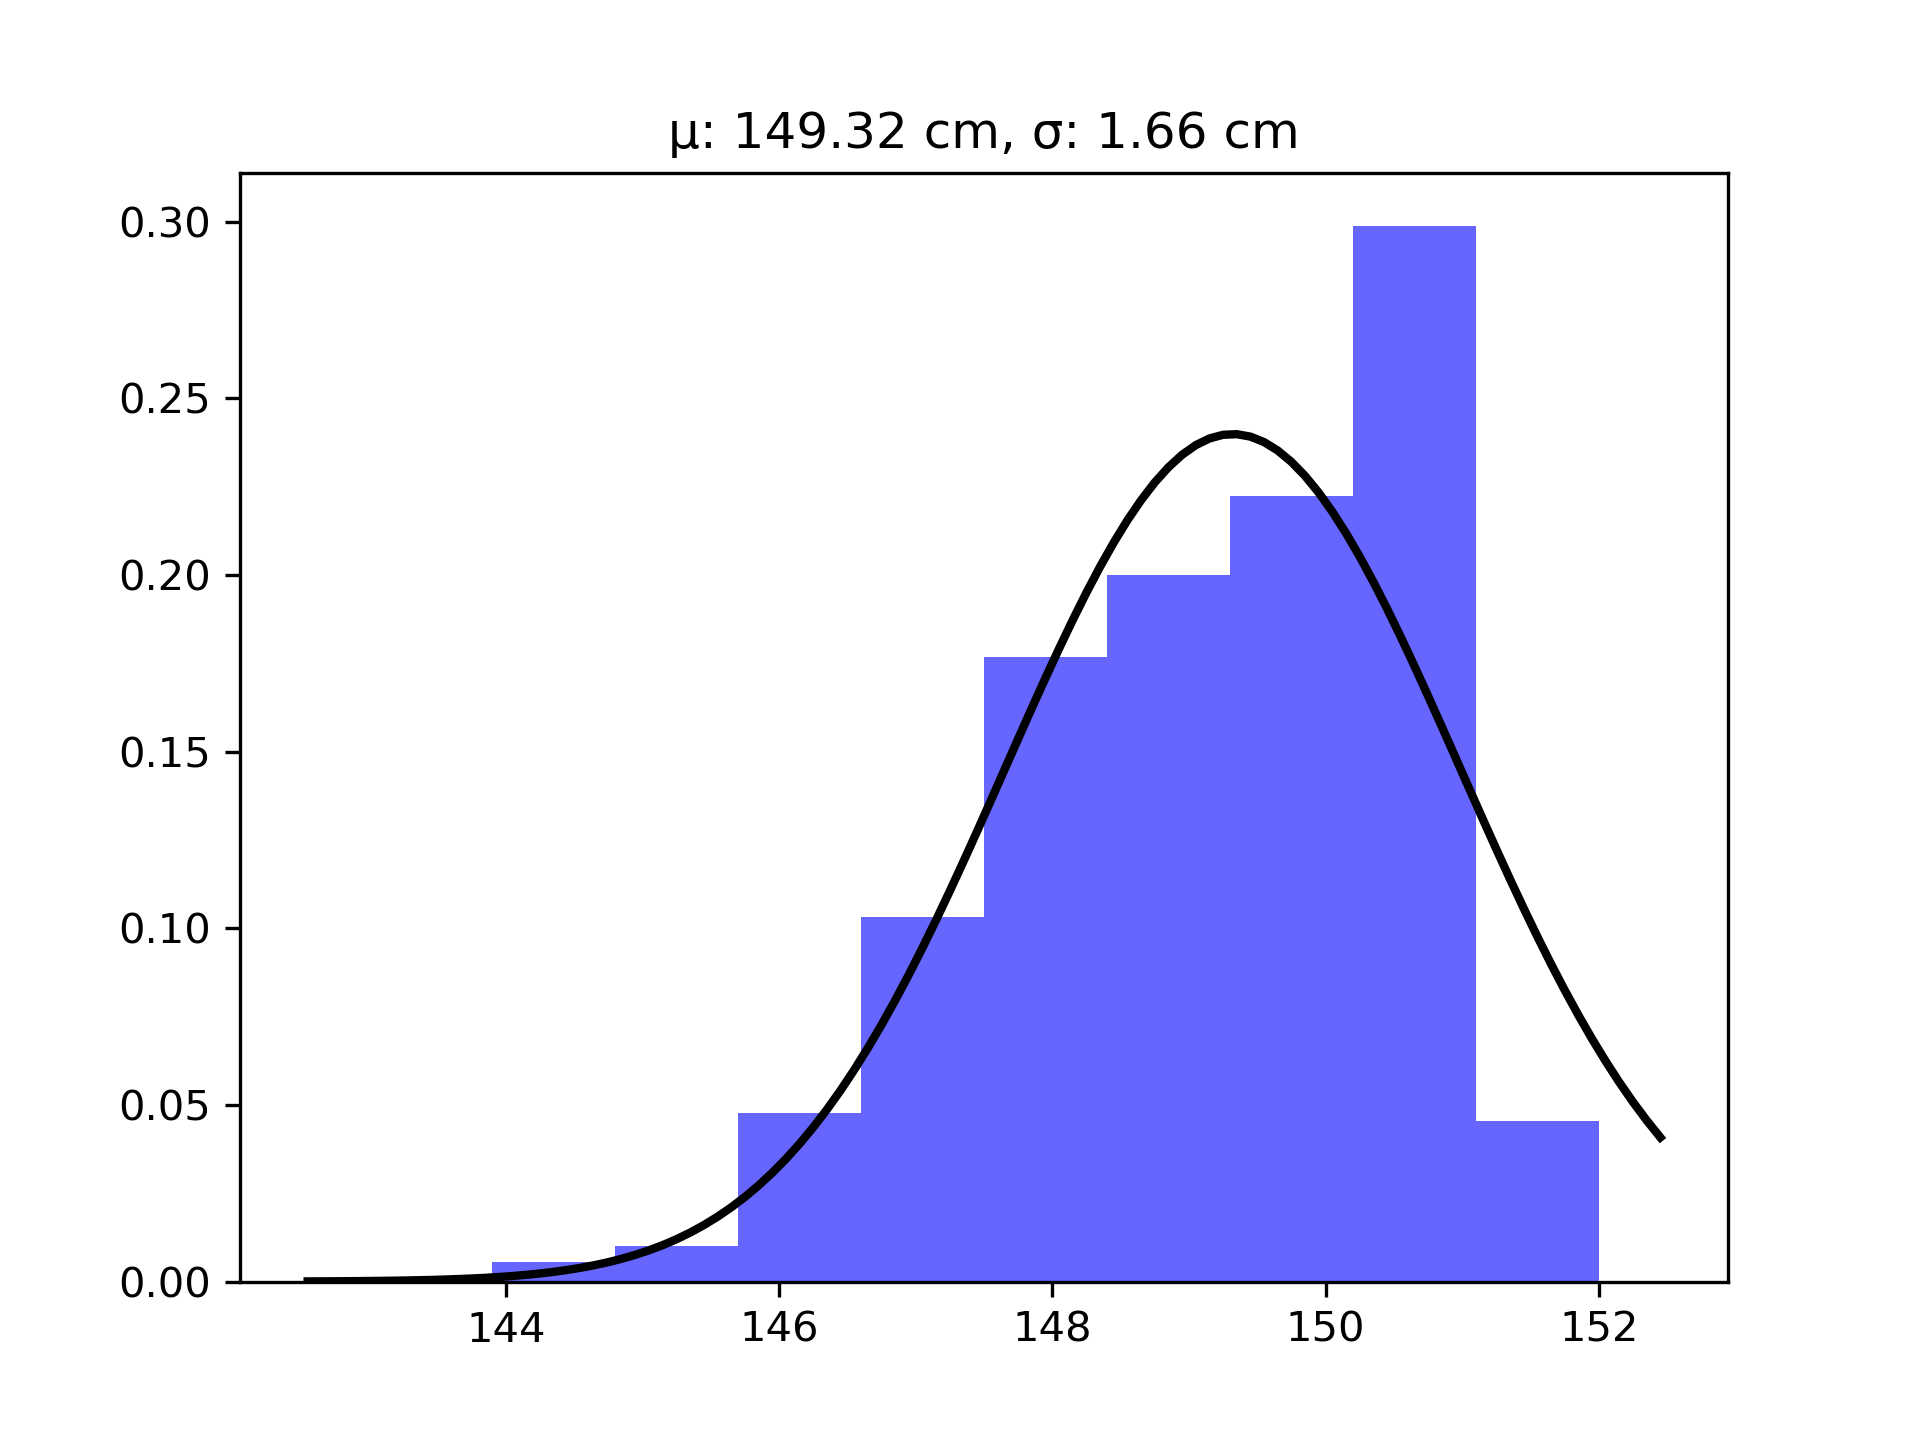
\includegraphics[width=0.45\textwidth]{images/ch5_range_hist.png}
    \caption{Channel 5 range measurements distribution at $+15$ degrees and $200$ centimeters}
    \label{UWB:fig:Range_ch5}
\end{figure}

\paragraph{Performance for height change}
in our Leader-follower application, the angle estimation robustness against the height difference between leader and follower, is an important requirement. Indeed in our application the target is supposed to be a ground robot, so the tag is placed at a low height. To asses the kit performance at different height, we have placed the target antenna at 3 different heights $h=[46,60,115]$ centimeters and at different angles $\alpha = [0,-30,-60,-75]$ degrees. The result are exposed in \autoref{UWB:fig:ch9_heights}. It can be seen that the height difference does not remarkably change the measured angle. Only for the measurements at $-75$ degree the measures are bad but, as previously stated, this is an angle related behaviour, so it does not invalidate this test outcomes.\\

\begin{figure}
    \centering
    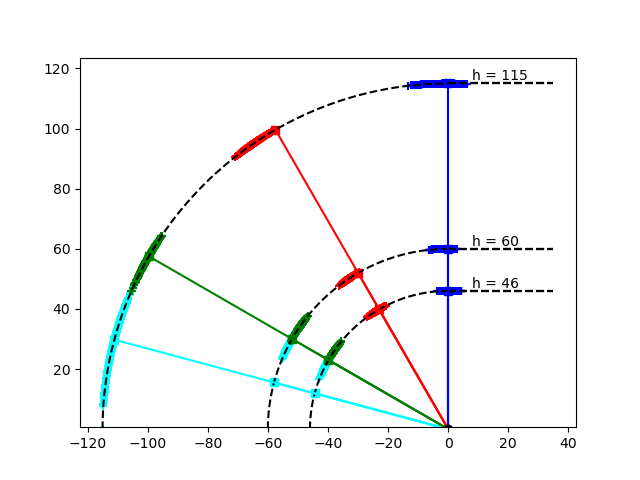
\includegraphics[width=0.48\textwidth]{images/ch9_heights.png}
    \caption{Angle measurements at different heights and at a constant x-y distance of $200$ cm.}
    \label{UWB:fig:ch9_heights}
\end{figure}

\paragraph{Behind the double UWB results}
in order to fully understand the sensor behaviour in different situations, a test with the target antenna behind the the double at a distance of $1$ meter was conducted. The results, together with the equivalent measure at one meter taken in front, are presented in \autoref{UWB:fig:ch9_behind}. As expected, given the manufacturer indication, the measure behind are quite chaotic, and both angles and ranges are mostly wrong. Even the data clouds are spread differently not resembling the constant behaviour seen for the front taken measures.

\begin{figure}
    \centering
    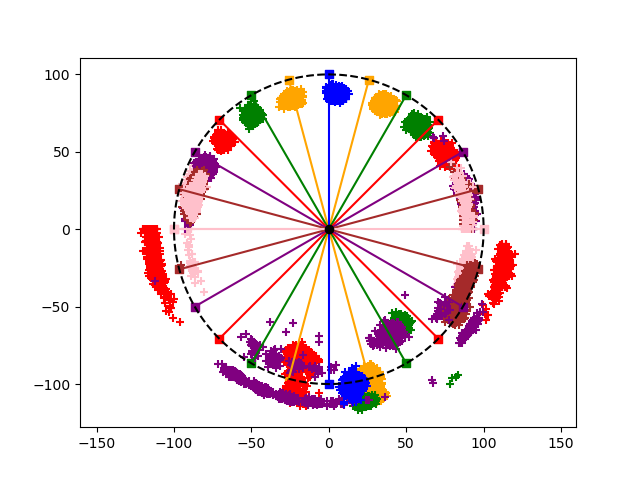
\includegraphics[width=0.48\textwidth]{images/ch9_behind_measure.png}
    \caption{Localization comparison between front and behind taken measures, expressed in centimeters.}
    \label{UWB:fig:ch9_behind}
\end{figure}

\paragraph{Conclusions}\label{UWB:conclus}
This evaluation kit has the potential to became a valid tool in Leader-follower applications, but some extra work on the sensor is needed. The main drawback is that the angle offset is a non linear function of the distance, and for application in which a dynamic range change is involved, this UWB pair is not suitable. To compensate for this behaviour, some work in modeling this offset's non-linearity is suggested. For what concern our purposes, this kit is precise enough, since in the region of interest (i.e. at $1.5$ meters $\pm 15$ degrees), it works pretty well. Even in the case of having wider angle and distances, since localization maintain his sign (e.g. if the true angle is $60$ degree, it measure $45$ not $-45$), our policy tends to converges towards the $0$ degree angle and $1.5$ meters distance, and so even in the presence of large accuracy error, the quadcopter is still somehow able to perform decently. Another modification effect on the measures noticed , that is not presented in this characterization, is the change in localization given by the relative orientation between the antennas. Indeed the best measures are obtained if the tag is placed radially w.r.t. the double, whereas important angle errors can be introduced if this condition is not respected (especially at short distances). This can overall truly impact the localization performance. In the real test, whose results will be later exposed, this last behaviour is surely responsible for a great amount of the localization error.